\documentclass[12pt]{article}
\usepackage{url, graphicx}

% page layout
\setlength{\topmargin}{-0.25in}
\setlength{\textheight}{9.5in}
\setlength{\headheight}{0in}
\setlength{\headsep}{0in}

% problem formatting
\newcommand{\problemname}{Problem}
\newcounter{problem}

% math
\newcommand{\dd}{\mathrm{d}}

% primary units
\newcommand{\rad}{\mathrm{rad}}
\newcommand{\kg}{\mathrm{kg}}
\newcommand{\m}{\mathrm{m}}
\newcommand{\s}{\mathrm{s}}

% secondary units
\renewcommand{\deg}{\mathrm{deg}}
\newcommand{\km}{\mathrm{km}}
\newcommand{\mi}{\mathrm{mi}}
\newcommand{\h}{\mathrm{h}}
\newcommand{\ns}{\mathrm{ns}}
\newcommand{\J}{\mathrm{J}}
\newcommand{\eV}{\mathrm{eV}}
\newcommand{\W}{\mathrm{W}}

% derived units
\newcommand{\mps}{\m\,\s^{-1}}
\newcommand{\mph}{\mi\,\h^{-1}}
\newcommand{\mpss}{\m\,\s^{-2}}

% random stuff
\sloppy\sloppypar\raggedbottom\frenchspacing\thispagestyle{empty}

\begin{document}

\noindent
Name: \rule[-1ex]{0.55\textwidth}{0.1pt}
NetID: \rule[-1ex]{0.2\textwidth}{0.1pt}

\section*{NYU Physics I---Term Exam 1}

\paragraph{\problemname~\theproblem:}\refstepcounter{problem}%
(From Problem Set 1, Problem~3)
Combine a mass $M$ and a length $h$ and an acceleration $g$ into
something that has units of time. You don't have to use all three
quantities if you don't need to.

\vfill

\paragraph{\problemname~\theproblem:}\refstepcounter{problem}%
(From Problem Set 2, Problem~3)
Make a plot of the velocity $v_y$ against time $t$ for a stone thrown upwards
at speed $v_y = +5\,\mps$. Use as the acceleration due to gravity $a_y = -10\,\mps$.
Plot for the time interval $0<t<1\,\s$.
Label your axes with sufficient precision that I can check your numbers.

\vfill

\paragraph{\problemname~\theproblem:}\refstepcounter{problem}%
(From Lecture, 2018-09-11)
We spent time talking about two vectors, $\vec{v}_3$ and $\vec{v}_4$,
which were the velocities of the rock on a no-air-resistance trajectory.
What was wrong with this picture, that we drew?
\marginpar{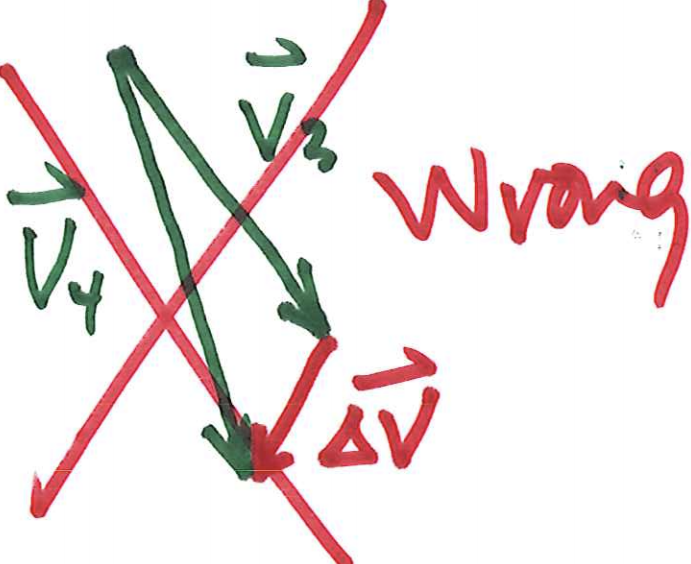
\includegraphics[width=1in]{../jpg/wrong_vectors.png}}

\vfill

\clearpage
\paragraph{\problemname~\theproblem:}\refstepcounter{problem}%
(From Lecture, 2018-09-13)
A car is moving at constant speed $v$ along a horizontal, circular path
of radius $R$. Is there a non-zero net force on the car? Why?

\vfill

\paragraph{\problemname~\theproblem:}\refstepcounter{problem}%
(From Lecture, 2017-09-18)
We gave three arguments that $g\,\sin\theta$ was a good guess for the
acceleration of a block down an inclined plane. The first argument was that it
has the right units! What were the other two arguments? \emph{Hint:} They were limiting
cases!

\vfill

\paragraph{\problemname~\theproblem:}\refstepcounter{problem}%
(From recitation, week of 2017-09-10)
You made a table of times, accelerations, positions, and velocities.
If in the third row you had
\begin{equation}
t_3 = 0.3\,\s
\quad
a_3 = -10.0\,\mpss
\quad
v_3 = -2.0\,\mps
\quad
x_3 = 9.7\,\m
\quad ,
\end{equation}
then what would you write for $v_4$ in fourth row, which looks like
\begin{equation}
t_4 = 0.4\,\s
\quad
a_4 = -10.0\,\mpss
\quad
v_4 = \rule[-1ex]{20pt}{0.1pt}\,\mps
\quad
x_4 = \rule[-1ex]{20pt}{0.1pt}\,\m
\quad ?
\end{equation}

\vfill
~
\end{document}
